\subsection*{Adaptive Control}
	\begin{figure}[H]
		\centering
		\begin{tikzpicture}
			\robotbase
			\angann{\thetaone}{$\theta_1$}
			\lineann[0.7]{\thetaone}{\Lone}{$L_1$}
			\link(\thetaone:\Lone);
			\joint
			\begin{scope}[shift=(\thetaone:\Lone), rotate=\thetaone]
				\angann{\thetatwo}{$\theta_2$}
				\lineann[-1.5]{\thetatwo}{\Ltwo}{$L_2$}
				\link(\thetatwo:\Ltwo);
				\joint
				\begin{scope}[shift=(\thetatwo:\Ltwo), rotate=\thetatwo]
					\grip
				\end{scope}
			\end{scope}
		\end{tikzpicture}
		\caption{2-Link Robotic Manipulator}
		\label{fig:manip2link}
	\end{figure}

	\begin{figure}[H]
		\centering
		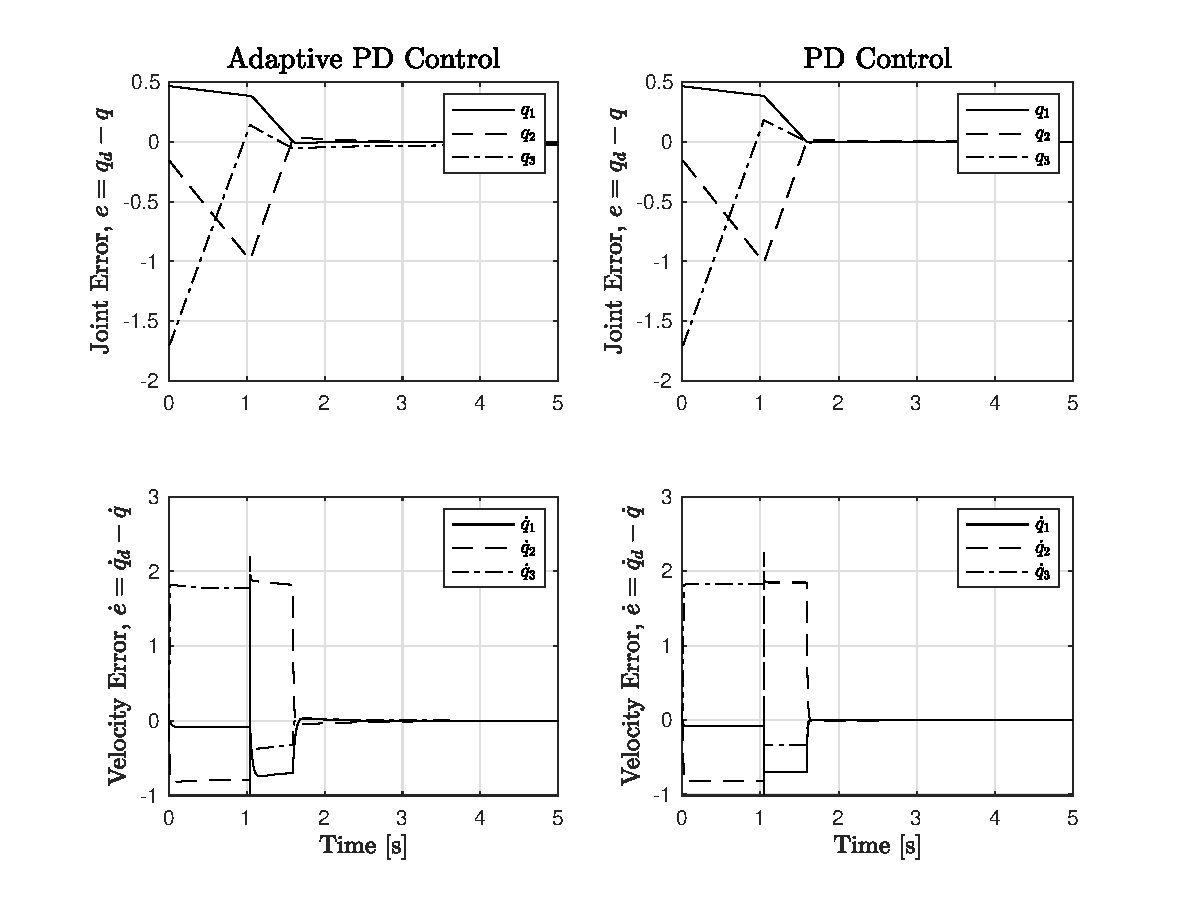
\includegraphics[width=0.7\textwidth]{figures/adpdErr.eps}
		\label{fig:adpdErr}
		\caption{Error Dynamics}
	\end{figure}

	\begin{figure}[H]
		\centering
		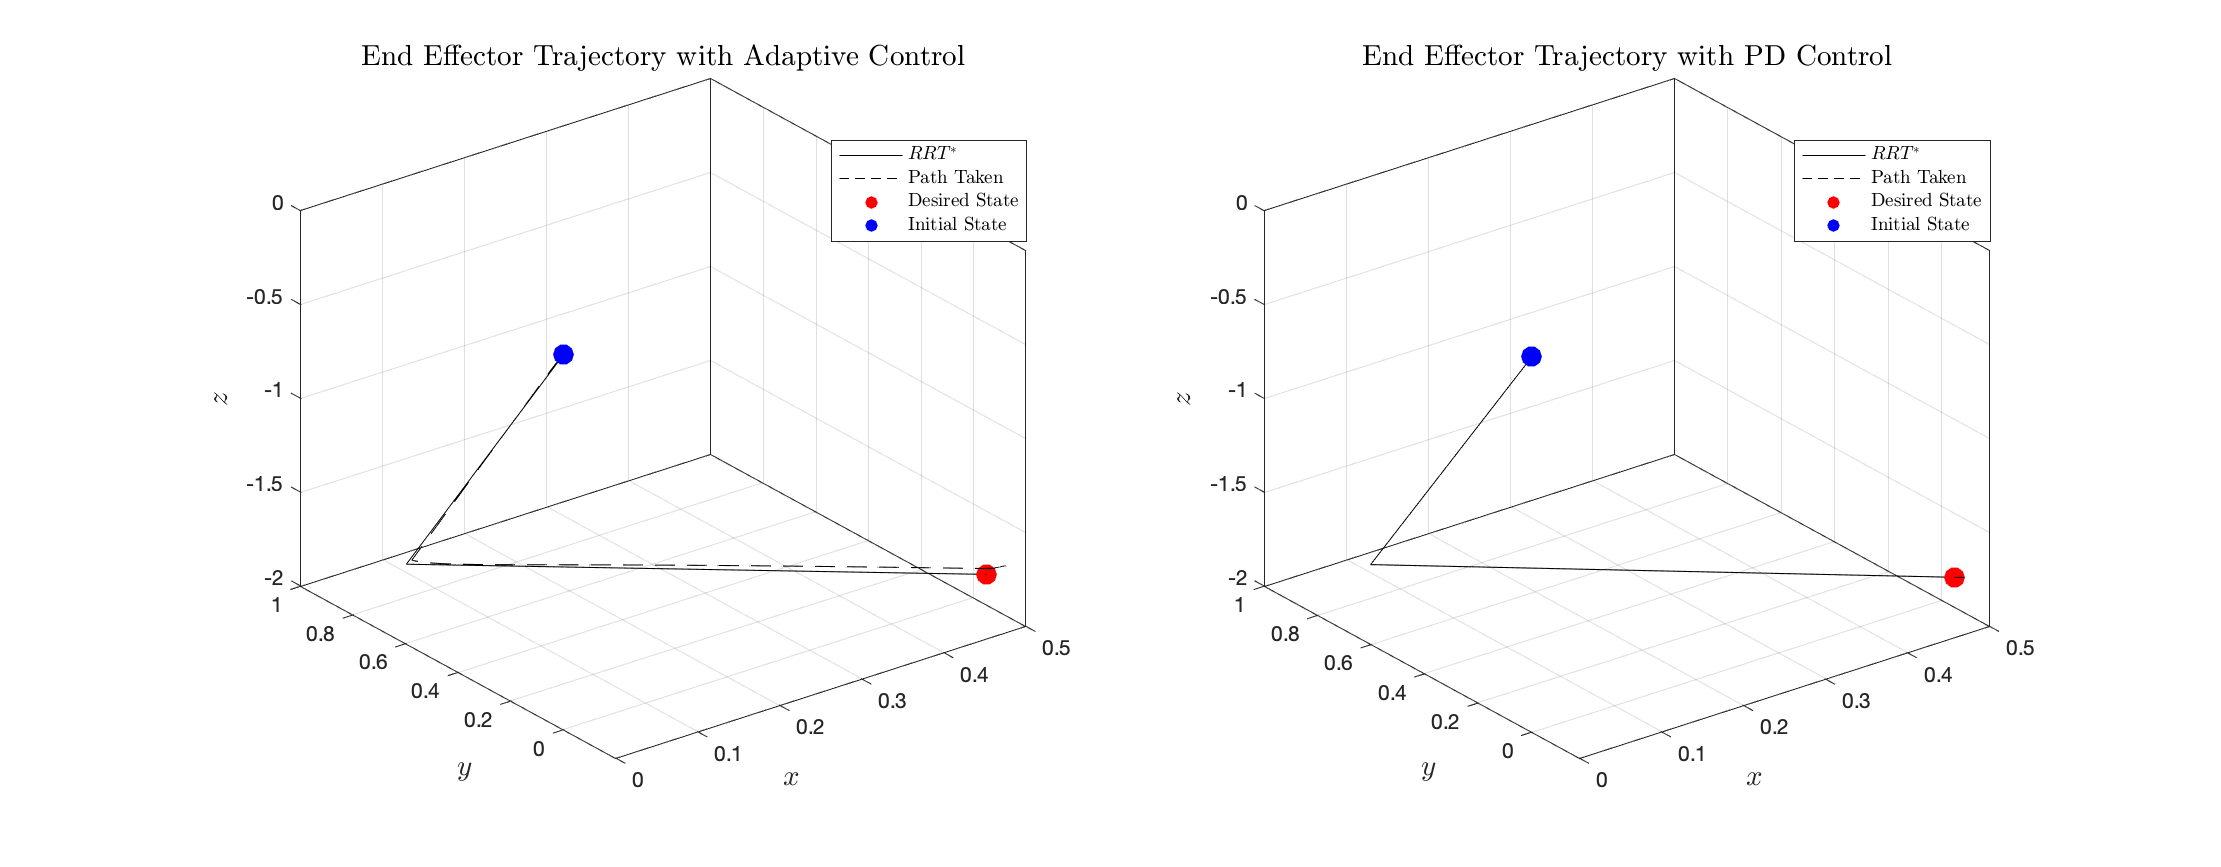
\includegraphics[width=0.9\textwidth]{figures/eeTraj.eps}
		\label{fig:eeTraj}
		\caption{End-effector trajectory}
	\end{figure}

	\begin{figure}[H]
		\centering
		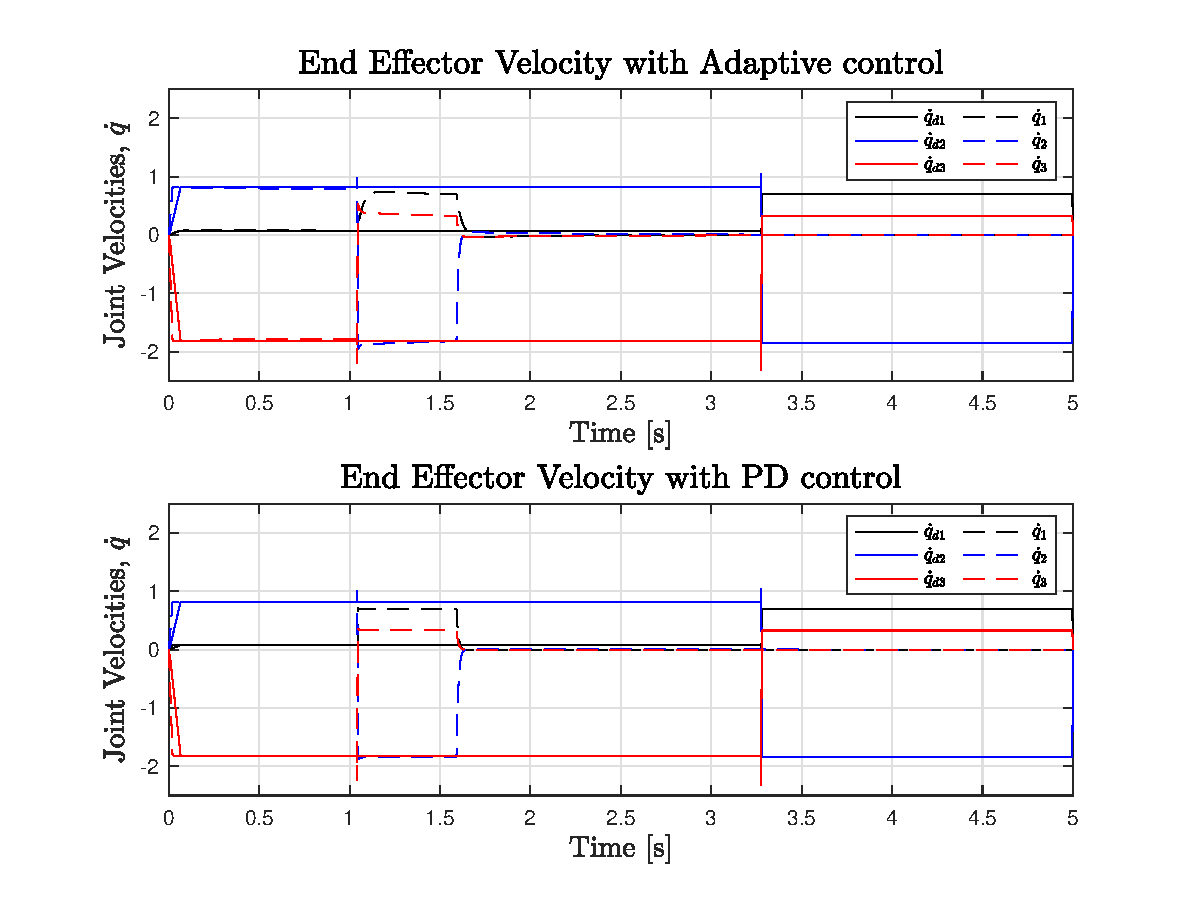
\includegraphics[width=0.7\textwidth]{figures/eeVel.eps}
		\label{fig:eeVel}
		\caption{End-effector velocities}
	\end{figure}

	\autocite{lewis2003robot}
